
\begin{abstract}
% Breiflydescribeintroductionto the topic, whatis the gab, aim, approach, and results
Her stal der stå et stykke abstrakt tekst.

This is a research project which aims to address the challenges of integrating systems in middleware within an Industry 4.0 environment. Using the case of developing an ammunition production line, the process entailed a systematic approach, utilizing appropriate tools to guide architectural decisions and system design, to ultimately render a solution that enables control of such production line. The paper covers how various tools (e.g. SysML, AADL, EAST-ADL, UPPAAL, CTL) and frameworks (such as Use Cases, Quality Attribute Scenarios (QAS), GQM) were utilized, along with a discussion of formal verification and validation (V\&V) and formal design.

\end{abstract}

\section{Introduction \& Motivation}
\label{sec:introduction}
% Introduction and motivation to the problem domain

% Der står en del omkring motivation i lecture_1_introduction slides
% Lecture_1_complex_systems indeholder noget omkring I4.0 og challanges

% Fra notion
This paper reports on and examines the results of the task of building a new software middleware system for an industry 4.0 production line of (rifle) ammunition for sport and hunting. The middleware will be able to exchange and coordinate information to execute and change a production. The software is going to be continuously deployable and run 24/7.

The system uses sensors to measure ammunition along the production line, as well as being able to change the production process in real-time for different ammunition types.

The focus of the case is to \textbf{integrate} the sensors and machinery, with the central system already in place at the factory. Due to the type of production line, \textbf{precision}, \textbf{safety}, 
% \textbf{security} 
and \textbf{performance} are very important considerations for the system.  

Moving forward, it is expected that the production line is \textbf{scaled} to multiple lines that run in parallel.

\section{Problem, research question \& approach} % Mikkel
\label{sec:problem-research-question-approach}
% What is the problem* to be solved with the reliable architecture you build, and how will the problem be addressed. *The stated problem leads to the stated research question
% Husk approach til hvordan vi kommer til at lave det

The current state of Industry 4.0 is challenged by the integration of systems. As uncovered by Jepsen et al. in \cite{Jepsen2020}, SDU's I4.0 lab is currently challenged with integrating the systems, as some systems are not ready for integration. This project therefore focuses on how a middleware system can be built for an I4.0 production line in the context of an ammunition production line. The middleware is abstracted away from the individual sensors and systems. It will therefore not focus on the currently lacking external interfaces of systems, but on how systems with integration options can be put together, using a middleware system. The project will also focus on the attributes needed for a production line, including integration, precision, safety, performance and scalability.

\subsection{Research Questions} \label{sec:research-question}
To ensure that our focus is placed correctly for our analysis, we use \textbf{research questions} that help clarify what task we need to solve:
\begin{enumerate}
    \item What architectural patterns can achieve a seamless integration in a production line with middleware?
    \item How can a system be designed to scale across multiple parallel production lines while maintaining performance and reliability?
\end{enumerate}

% Usikker på hvad vi kunne have her
% Vores opgave er at lave en productions line som passer ind i industry 4.0.
% Den skal overholde forskellige QA
% på basis af overståen lav 2-3 RQ. de må gerne være simple


\subsection{Approach}

To create a suitable I4.0 middleware system, a heavy focus will be put on the architecture of the system. Specifically, there will be a large focus on the quality attributes, as well as the interaction between elements. Identified requirements will be mapped to the quality attributes and tactics and patterns will be found to correctly tackle and fulfill these quality attributes. Feature modeling will be used to model the possible features, as well as their relation. ADL, AADL, EAST-ADL will be used to model the system to understand and evaluate it. UPPAAL will be used to model the states in the system, in order to evaluate if the behavior is possible. This consolidates into a formal validation and verification on the project.
In order to ensure the system can be built in regards to its requirements, experiments will be conducted in critical areas.

\section{Related work}
\label{sec:related-work}
% The related work should review the state of the art consisting of 8-10 papers and should contextualize how this study provides new knowledge to the field. Here you can combine  the work from scientific methods
% Det her burde være kort (lad det være det sidste)
% Hvordan bruges det fremad?
In order to have a good starting point and build upon the existing knowledge space, it is important to first investigate what the state of the practice is in the field. Therefore, during this project, we have conducted a literature review to identify and review studies that relate to our research questions and topics. This can provide credibility to the claims we make and valid reasoning about the decisions we make. 


% By doing this we can base our research project on existing studies that will help validate our project. The studies we base our research on will be cited to reinforce the statement of our claims and give us credibility. It is therefore important that we are careful when finding sources within the relevant areas.

We have largely utilized the primary study by Jepsen et al. \cite{Jepsen2020} to build our knowledge and support our reasoning, as alluded to in Section \ref{sec:problem-research-question-approach}.

% For this project, we have built our knowledge on a primary study by \cite{Jepsen2020} read \ref{sec:problem-research-question-approach}.

Studies by T. Borangiu and S. Răileanu \cite{Borangiu2020} explain the role of middleware within cyber-physical systems for real-time monitoring of data integration. They recommend a decentralized system that does not limit the decision-making process but uses entities and channels that transport data and information.

\section{Use cases}
\label{sec:use-case}
% Unfold the problem with a use case and describe what the use case is about.

% Lecture 2 exercises, viser mere omkring dette.

% Use case diagrammer og lignende
% Hvordan bruges det fremad / Hvorfor har vi det (meget kort)
Use case diagrams is a behavioral diagram (see Figure \ref{fig:structural-diagram}), that allows stakeholders to get a understanding of how the system is intended to behave. By creating use case diagrams we are able to define an overview of the process and formulate requirements. 

In order to understand the case, a number of use cases have been elicited. These use cases serve as the project's backbone, as they list how the final product should function.

For this project, two main stakeholder groups have been identified: production managers, who are responsible for the production line and production orders, and machine operators, who handle the individual machines regarding maintenance and faults.

% !! Har udeladt Business values, fordi jeg ser ikke nogen grund til dette

In order to produce the use cases several assumptions of the system have been made.

Part of a larger corporation, the factory is in charge of producing the corporation's offering of \textit{2} different types of ammunition: \textit{Rifles} and \textit{pistols}. 
The factory has \textit{5} production lines capable of producing all types of ammunition.
The production facilities include \textit{15 sensors} and \textit{5 different robots} for each production line.
The main challenge of this department is to \textit{integrate sensors and robots} into a \textit{unified system} that can integrate with the ERP system to dispatch productions.

The process of manufacturing is; to first get ammunition casing, then place ammunition casing on track. Get primer
and insert primer into the ammunition casing. Get propellant and put in propellant into casing. Get ammunition head and insert ammunition head into ammunition casing. Get a package to pack ammunition into it and insert ammunition into the package, then close the package with ammunition in it and store packages in the warehouse. This results in a 12-step process.
The moving of products to and from the production line is handled by a single system. Another system already exists for ordering material, the system to be built will therefore integrate with these systems.

Four use cases have been created. Use Case 01 (UC01) is the primary use case for the system, and includes production initialization. The use cases can be seen in the Appendix as Figure \ref{fig:appendix-use-case-01}. Use cases for "Real-Time Monitoring and Control of Production Line", "Automated Quality Control and Defect Detection" and "Handling System Failures on the Production Line" have also been produced as use cases UC02, UC03 and UC04 respectively.

\subsection{Requirements}
Requirements are created by analyzing the description introduced in Sections \ref{sec:introduction}, \ref{sec:problem-research-question-approach} and \ref{sec:use-case}, this is done in order to create the functional and non-functional requirements. These requirements will help to form the classes and describe what the expectations for the architecture is in form of quality attributes (QA).

Due to the project's structure of components, requirements for each of the different systems and their subsystems were created as individual entities. This division helped to maintain the overview and allow all systems to be developed individually without being dependent on each other. 

% Each requirement was given an ID that is used to refer to the requirements.

A selection of the functional and non-functional requirements for the \textbf{MES} subsystem can be observed in Table \ref{tab:mes_functional} and \ref{tab:mes_nonfunctional}.

\begin{table}[H]
    \centering
    \caption{Functional Requirements for MES}
    \label{tab:mes_functional}
    \begin{tabular}{|c|p{6cm}|}
        \hline
        \textbf{ID} & \textbf{Functional Requirements} \\
        \hline
        F1 & Interface for receiving tasks for the production. \\
        \hline
        F2 & Report back to the user if alerts in requested tasks. \\
        \hline
        F3 & Retrieve data regarding production speed, machine status, and downtime. \\
        \hline
    \end{tabular}
\end{table}

\begin{table}[H]
    \centering
    \caption{Non-Functional Requirements for MES}
    \label{tab:mes_nonfunctional}
    \begin{tabular}{|c|p{6cm}|}
        \hline
        \textbf{ID} & \textbf{Non-Functional Requirements} \\
        \hline
        NF1 & Task determination to execution, must be delivered to the robot system within 500 ms. \\
        \hline
        NF2 & Must scale in sync with the production line. \\
        \hline
        NF3 & Must have an up-time of 99.999\% and be available 24/7. \\
        \hline
        NF4 & Must support continuous deployment, ensuring the system does not go down during software updates. \\
        \hline
    \end{tabular}
\end{table}

\section{Quality attributes} \label{sec:quality-attribute-scenario}
% The use case is the foundation to describe and specify architectural requirements.
% Quality Attributes hvad er det hvorfor har vi det hvordan bruger vi dem. 
Quality attributes are the desired traits of a given system. 
% and guides architectural decisions, in an aim to best achieve them. 
They are articulated as the non-functional requirements of an architecture. They help guide architectural design decisions to ensure that the legal and stakeholder non-functional requirements are met.
%They are used to ensure that the system meets current and future needs and help guide design decisions by evaluating the various requirements.
%These requirements are achieved using patterns and tactics.

The quality attributes that will be the focus of this project are defined based on our research questions (see Section \ref{sec:research-question}), use cases (see Section \ref{sec:use-case}) and the systems non-functional requirements (see Table \ref{tab:mes_nonfunctional}), and are as follows:
%The following QA's are defined with a focus on Research questions.
\begin{itemize}
    \item \textbf{Integrability} the ability of the system to work together with other systems across existing or new systems.
    \item \textbf{Modifiability} is about the system being able to be changed quickly to handle requirements or errors that arise.
    \item \textbf{Performance} is the ability of the system to perform its functions quickly and efficiently.
    \item \textbf{Availability} is the system's ability to be operational and available to the processor.
     \item \textbf{Scalability} is the ability of the system to handle load increases without decreasing performance, or the possibility to rapidly increase the load.
\end{itemize}



% flyt krav her op


% lav quality attributes scenario hvad er det hvorfor har vi det hvordan bruger vi dem. det skal baseres på experimentet, så det kunne være safety 
\subsection{Quality Attribute Scenarios}
To better understand quality attributes, we describe them using Quality Attribute Scenarios (QAS). They describe the requirements in a systematic and verifiable manner that helps provide understanding for all stakeholders in the project.

\begin{figure}[H]
    \centering
    \caption{\centering Quality Attribute Scenarios (QAS) \\ Six elements that define the scenario}
    \label{fig:qas-diagram}
    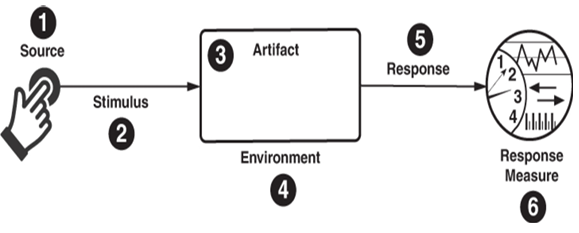
\includegraphics[width=0.93\linewidth]{report/GroupTemplate/images/qas.png} 
\end{figure}


The process of defining QAS' is by defining the six elements, see Figure \ref{fig:qas-diagram}.

\begin{enumerate}
    \item \textbf{Source}: who or what triggers the event
    \item \textbf{Stimulus}: the type of event that occurs
    \item \textbf{Artifact}: what part is affected
    \item \textbf{Environment}: defines the conditions under which the event occurs
    \item \textbf{Response}: the response to the event and 
    \item \textbf{Response measure}: how it is measured
\end{enumerate}

In this project, the following quality attribute scenario has been made for performance.

\begin{enumerate}
    \item \textbf{Source}: 15 sensors, with an order of 1000 ammunition rounds being produced
    \item \textbf{Stimulus}: Produces 300 sensor readings a second, total from all sensors
    \item \textbf{Artifact}: MES system
    \item \textbf{Environment}: Normal operations
    \item \textbf{Response}: Process and track each reading and match it to a specific round 
    \item \textbf{Response measure}: Average processing time of 200 ms.
\end{enumerate}

\subsection{Architectural Patterns and Tactics}
Tactics are the design decisions that explain how the quality attributes are used. The goal of a tactic can be the response to a stimulus by improving e.g. availability, see Figure \ref{fig:goal-availablity tactics}.
\begin{figure}[H]
    \centering
    \caption{Goal of Availability Tactics}
    \label{fig:goal-availablity tactics}
    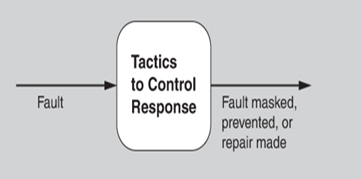
\includegraphics[width=0.5\linewidth]{report/GroupTemplate/images/Goal of availability tactics.png}
\end{figure}

Tactics allow patterns to be adapted to a specific area, and by using a systematic process, it is possible to reinforce patterns using these tactics.
Patterns focus on specific ways of implementing common software development solutions for common problems and do not directly link to quality attributes. Often, a single pattern may solve multiple tactics.

Figure \ref{fig:availability-tactics} shows different tactics that can be used to improve availability, shown via a tree diagram, branching out according to the different problems that one desires to address.

\begin{figure}[H]
    \centering
    \caption{Availability Tactics}
    \label{fig:availability-tactics}
    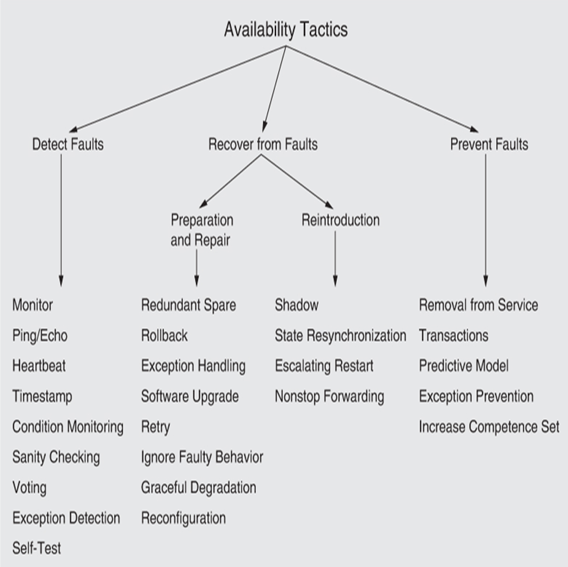
\includegraphics[width=0.7\linewidth]{report/GroupTemplate/images/Availability tactics.png}
\end{figure}

To get an overview of the architectural choices made for the different quality attributes, a questionnaire is created where questions are asked and they are recorded in a table. The answers to these questions can then be made the focus of further activities such as examining documentation, analyzing code or other artifacts, reverse engineering code, and so on.



% hvad er tactics hvorfor har vi det og hvordan har vi brugt det

% hvad er patterns hvorfor har vi det og hvordan har vi brugt det

% Forklar hvad forskellen på Pattern og Tactics er.
% Patterns er forklaret i lecture_3_design_patterns

% Forklar quality attributes, og quality attribute scenario (diagram)

\section{Design and Analysis Modeling}
\label{sec:design-and-analysis-modelling}

After establishing the requirements for the system, the next step is to design the system. In this process, it is important to analyse the system, in order to create a solid foundation for the project.
This section will therefore cover the design and analysis parts of the project, for the architecture and software.

% Describe the design and argue for the design decision and how it meets the QASes. Part of the design decision must specify which tactics/patterns are used (provide arguments) and the trade-offs.
% Analyze the design and illustrate the system architecture model, encompassing both structure and behavior, using formal reasoning.

% Der skal laves diagrammer under specifikke afsnit herunder 



% Er i notion, skal skrives ind. Requirements skal omhandle, Functional og non-functional. Udvælg de vigtigste, beskriv Hvorfor vi har det, hvad vi bruger det til og Hvordan vi har lavet det.
\subsection{Requirement Diagrams}

\textbf{Requirement diagrams} is able to bridge the gap between text-based requirements while it helps improve requirement management throughout the system by providing traceability between text-based requirements and the model elements that represent the system analysis, design, implementation, and test cases.

\begin{figure}[H]
    \centering
    \caption{\centering Requirement Diagram, giving a overview of the relations}
    \label{fig:requirements-diagram}
    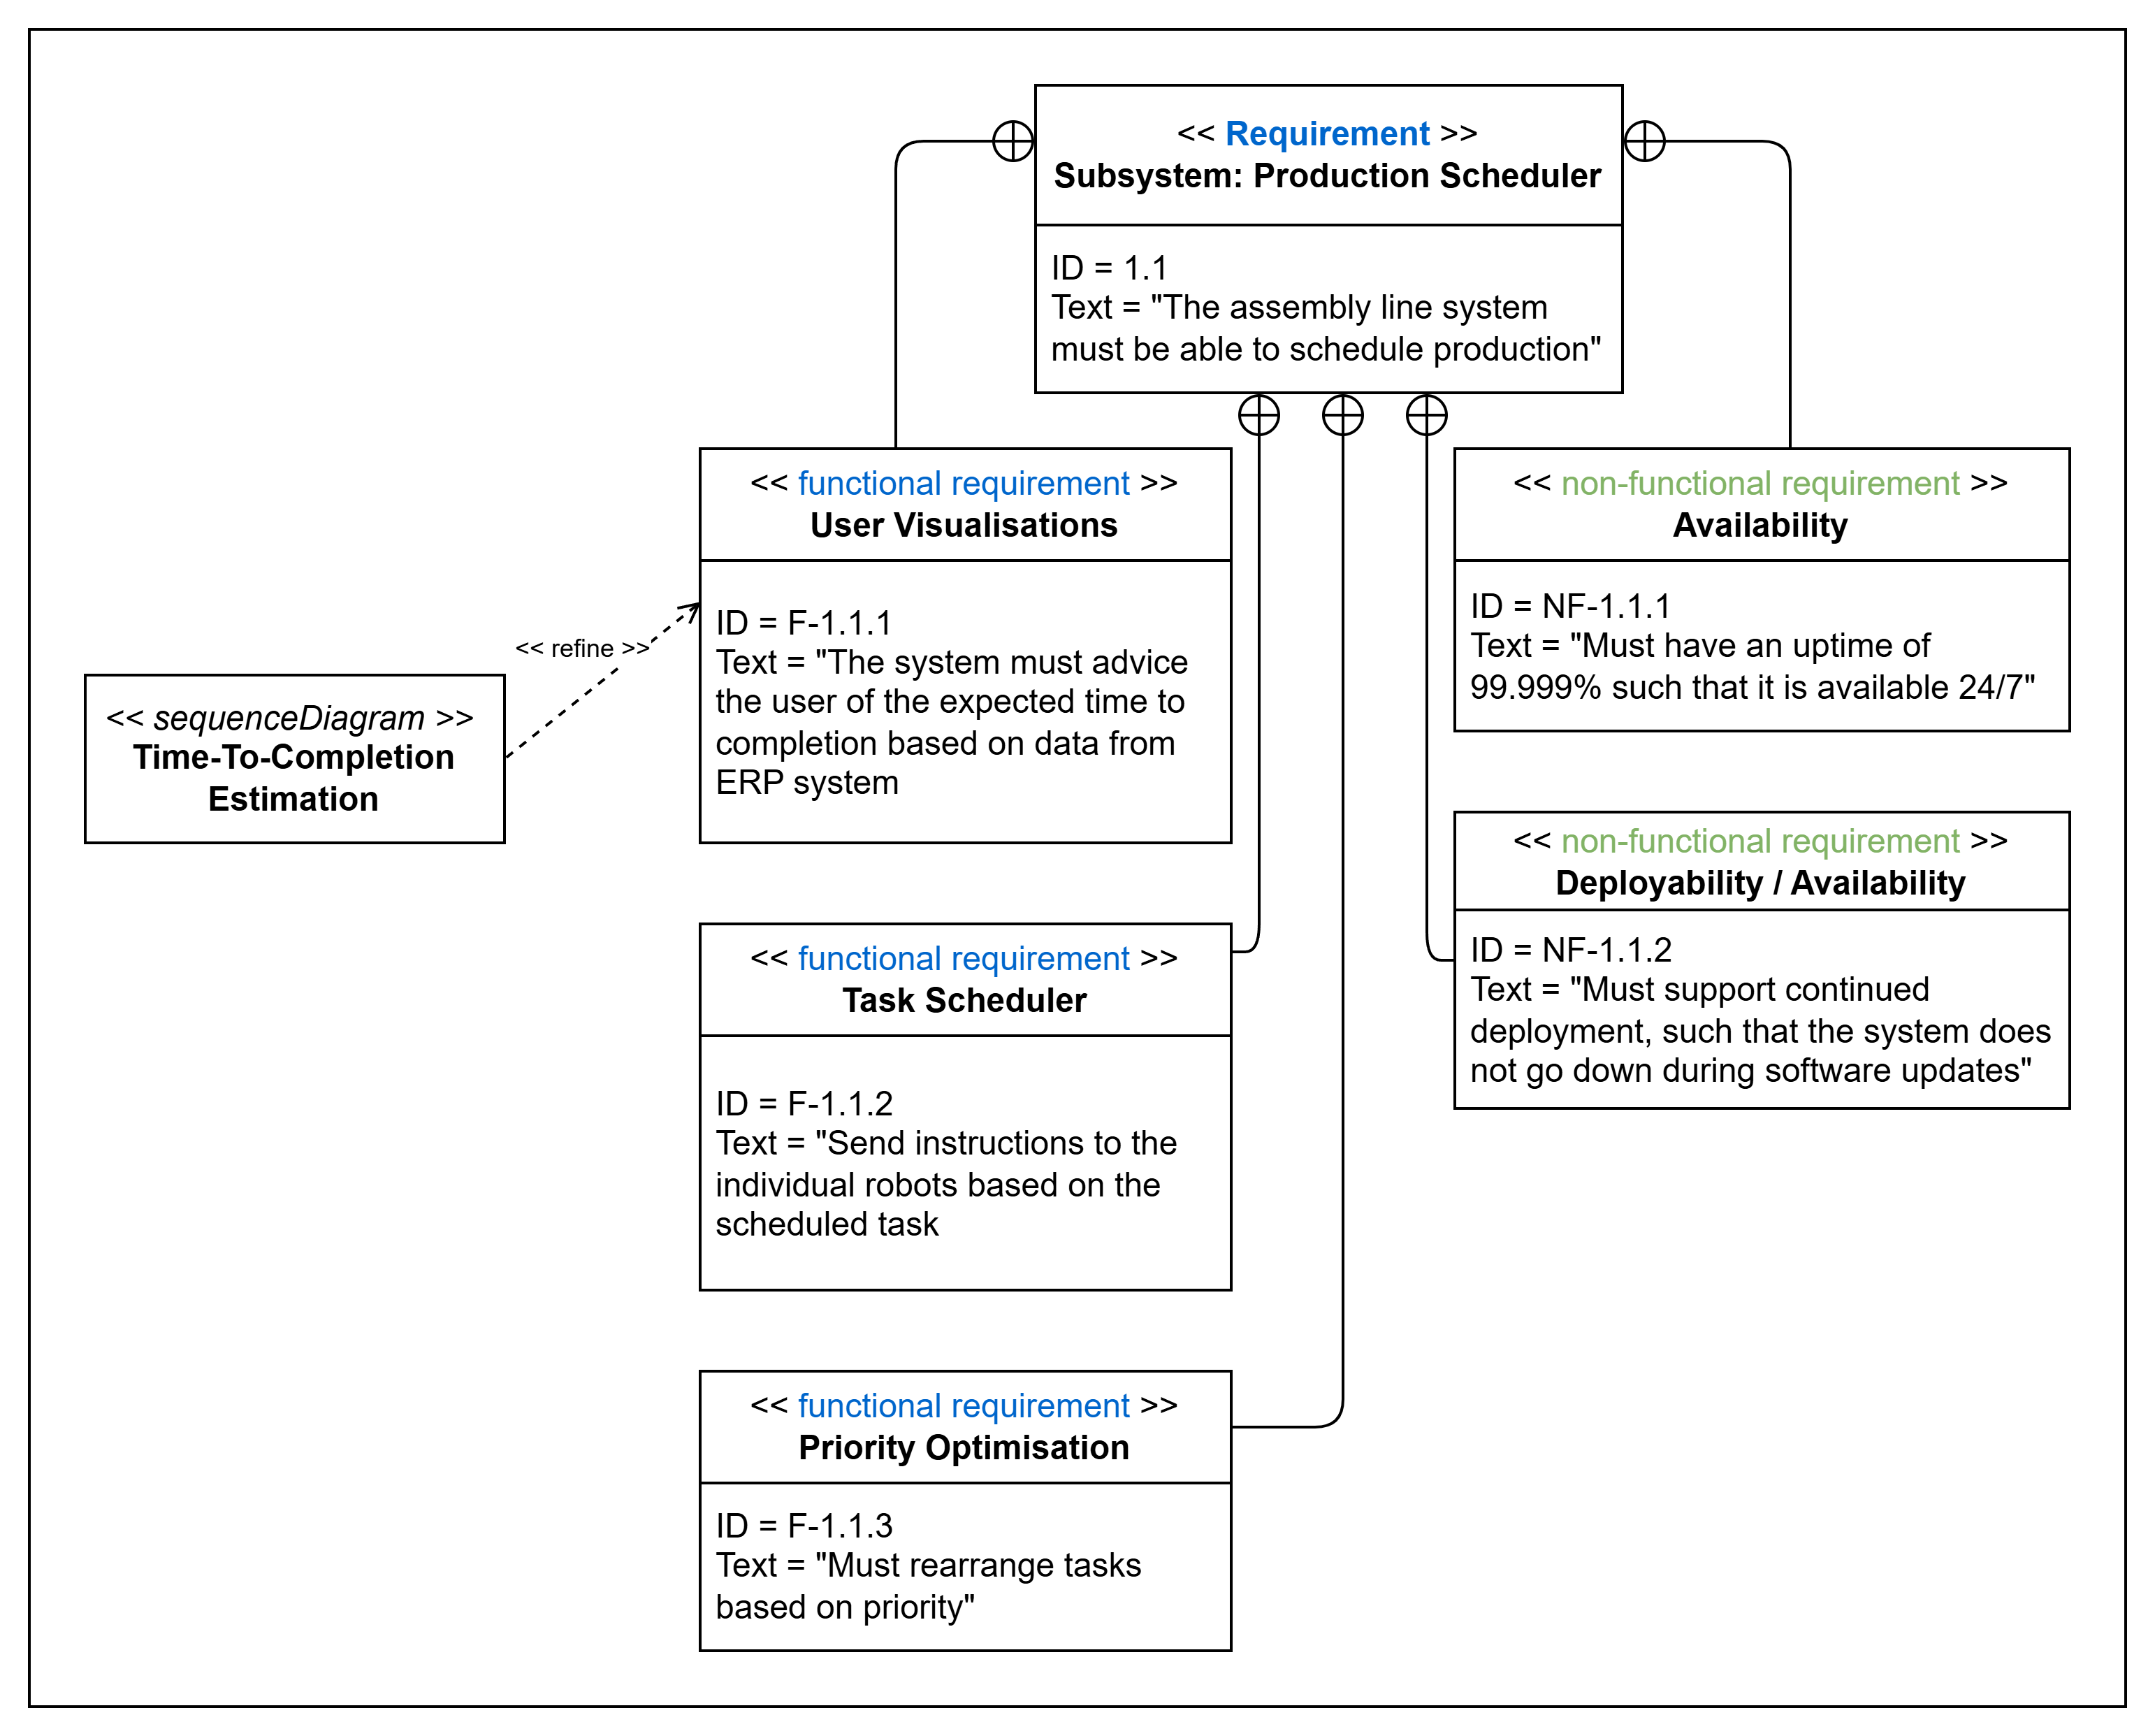
\includegraphics[width=0.9\linewidth]{report/GroupTemplate/images/requirements diagram.png}
\end{figure}

A requirement diagram, as seen in Figure \ref{fig:requirements-diagram}, is a static structure diagram that shows the relationship between our \textit{requirements} constructs, model elements that \textit{satisfies} dependency, and test cases that \textit{verify} dependency.
% mangler Refine, Satisfy, Verify, Trace og Copy relationship

The purpose of requirement diagrams is to specify both functional and non-functional requirements in the model so that they can be traced to other model elements that satisfy them, and test cases that verify them. All while providing a hierarchy and traceability between requirements.

\begin{figure}[H]
    \centering
    \caption{Requirements Utilize Basic Relations, \cite{WormKangLec72024}}
    \label{fig:requirement-diagram-relations}
    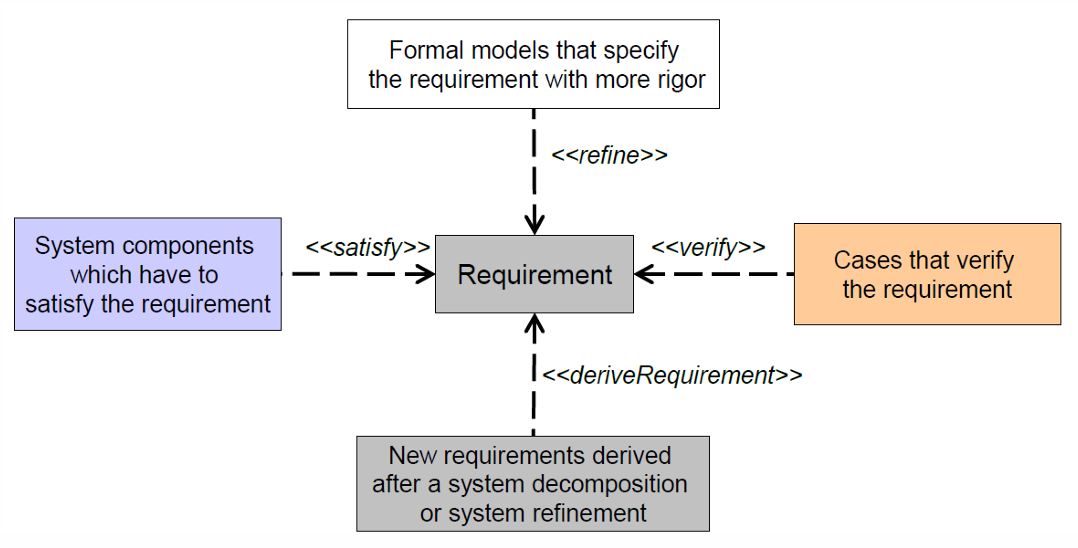
\includegraphics[width=0.9\linewidth]{report/GroupTemplate/images/Requirements basic relations.png}
\end{figure}
As stated by Eun-Young Kang:
\begin{quote}
The \textbf{refine relationship} in Figure \ref{fig:requirement-diagram-relations} is shown with a dotted line with the keyword \textit{refine} with the arrow pointing from the element representing the more precise representation to the element being refined.

The \textbf{satisfy relationship} in Figure \ref{fig:requirement-diagram-relations} is used to assert that a model element corresponding to the design or implementation satisfies a particular requirement. The actual proof that the assertion is true is established by the \textbf{verification relationship}. The \textbf{satisfy relationship} is shown by a dotted line with the keyword \textit{satisfy} with the arrow pointing to the requirement to assert that the block satisfies the requirement.

\textbf{Trace relationship} provides a general relationship between a requirement and any other model element. Useful for relating Reqs to source documentation or establishing a relationship between specifications. Shown as a dotted line with the keyword \textit{trace} with the arrow pointing to the source document.

\textbf{Copy relationships} support the reuse of Reqs by explicitly relating a copy of a Req to a source Req. The text property of the copied Req (slave Req) is a read-only copy of the text property of the source Req (master Req), but the copied Req has a different ID and may be contained in a different namespace. The copy relationship is shown by a dotted line with the keyword \textit{copy} with the arrow pointing from the copied Req to the source Req.
\end{quote}
\subsection{Feature Modeling} % Jon
% I lecture4-23-09-2024 er der mere omkring dette

% Beskriv hvad det er, og hvordan det bruges i projektet og hvorfor
% What is a Feature ?
% A Feature is a characteristic or trait that the variants of a variable entity may or may not have.
A feature model is a systematic way to represent and manage different features in a software product. % or software product line. 
The model is primarily used to organize and visualize the system's features in a hierarchy, where each feature can be mandatory, optional, alternative, or part of a group of features. The purpose of a feature model is to help software developers understand and structure the common properties of the system and the variations that can be found between different system variants\cite{featuremodels2023}.

\begin{figure}[H]
    \centering
    \caption{Feature Model Overview of Production Line}
    \label{fig:feature-model}
    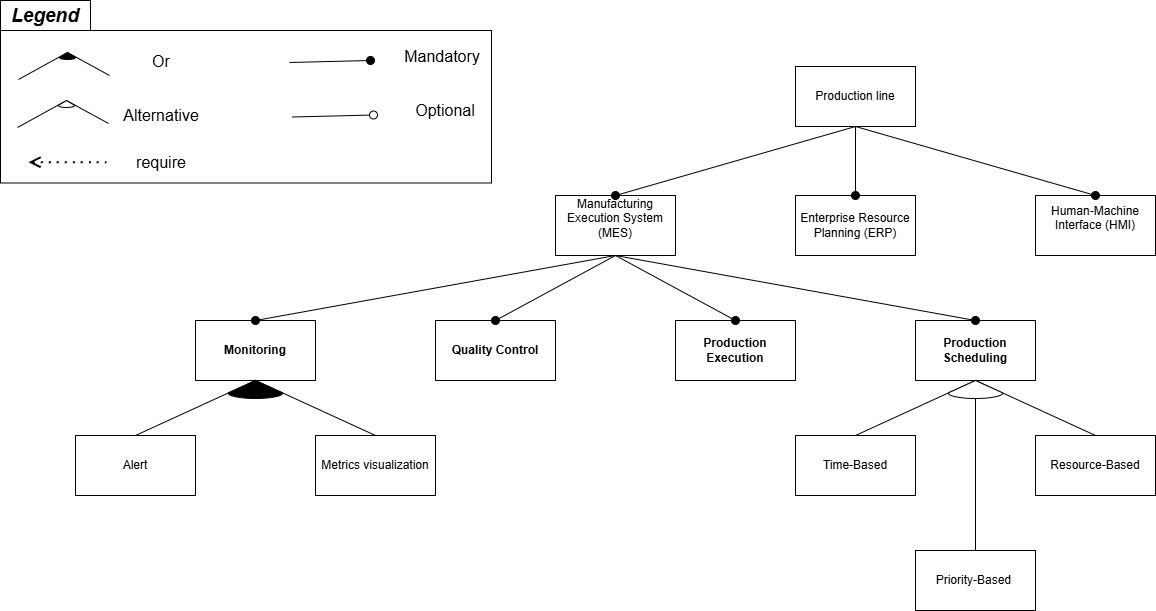
\includegraphics[width=1\linewidth]{report/GroupTemplate/images/feature_modelling.png}
\end{figure}

Figure \ref{fig:feature-model} shows an overview of the production line with its system, subsystems and their features and sub-features. The production line is the system that branches into three main subsystems, Manufacturing Execution System (MES), Enterprise Resource Planning (ERP), and Human-Machine Interface (HMI). These three subsystems are \textbf{mandatory}, indicating that they are essential components for the operation of the production line in all configurations. The \textbf{mandatory} indicators are depicted by a line with a filled bubble, while \textbf{optional} indicators are lines with hollow bubble.

Monitoring is a subsystem that contains the \textbf{features} "Alert", and "Metrics visualization", which represents different ways of extraction metrics from the system. They are connected to monitoring with an \textbf{OR} relationship, allowing for either one or both of the features to be present in the system.

In the production scheduling module the feature description allow for \textbf{alternative} methods of scheduling. These alternatives are represented by a feature marker \texttt{Time-Based}, \texttt{Resource-Based}, and \texttt{Priority-Based}. The alternative marker makes allows for either one to be present, but only one.

From Figure \ref{fig:feature-model} the \textbf{require} and \textbf{excludes} are not depicted. It is still important to know that the \textbf{require} relationships, indicates that one depends on the presence of another to function correctly. While the \textbf{excludes} indicate that two features or sub-features cannot coexist in the same configuration.

% Feature Leve/
% • A system is characterized by a set of Features.
% • Features are stakeholder requested functional or non-functional characteristics of a system.
% • A Feature describes that "what", but shall not fix the "how".
% • A Feature is specified by requirements and use cases.
% • From a top-down architecture approach the features are the configuration points to create a system variants.
% Indeholde diagram




\subsection{Systems and Subsystems} % Mikkel
\label{sec:systems-and-subsystems}

In order to facilitate the different operations the system is designed to, it has been identified that the system can be split into three different systems; Manufacturing Execution System (MES), Enterprise Resource Planning (ERP) and Human-Machine Interface (HMI). 
By doing this, the system is split into smaller systems, that different teams can work on. It also allows for the isolation of independent systems. 
By splitting it up, the final system is built as a micro-service architecture, as the individual elements are built and deployed independently of each other.

\begin{figure}[H]
    \centering
    \caption{\centering A High-Level Diagram Depicting the Overall Architecture of the System}
    \label{fig:systems_and_subsystems-system_diagram}
    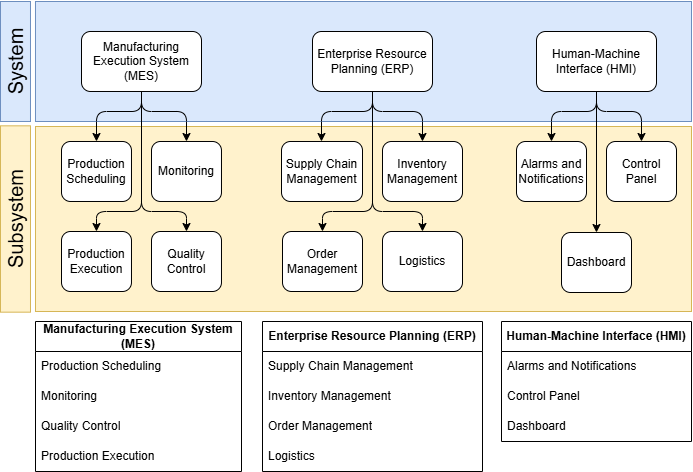
\includegraphics[width=1\linewidth]{report/GroupTemplate/images/Systems&Subsystems.png}
\end{figure}
% Systemer og subsystemer kommer fra exercise 3.1
% Beskriv systemerne


The splitting of systems, and identifying subsystems, also allows for better interoperability and inclusion of existing software solutions in parts of the final system.


In Figure \ref{fig:systems_and_subsystems-system_diagram} a diagram of the systems and subsystems can be seen.
Each subsystem in the diagram may be made up of smaller modules and already existing software solutions.

% Another possibility is starting by specifying the systems and subsystem, is that it serves as the base design for the architecture structure model.

With systems and subsystems identified, they serve as the base for the next step; the Architecture structure model.

\subsection{Architecture Structure Model} % Mikkel
\label{sec:architecture-structure-model}
%ASL - Vores store diagram med alle vores submoduler

In order to understand the system and be able to communicate about it, an architecture structure model can be made.
The architecture structure model, is a model that represent the structure of the architecture. Being close to the Component \& Connector (C\&C) diagram type, architecture structure model is unique, in that it focuses on the high level structure of the application. The architecture structure model is an informal diagram type, and can be shaped to the level of details needed for the communication and documentation of the overall structure of the architecture.

In this project, the architecture structure model focuses on the individual systems, what elements are used and how they interact with other systems and pre-made elements. The model has allowed for discussion of the structure of the application, and how different systems interact. The architecture structure model has been split into three diagrams, which together form the full system. The diagrams are for each system in the project; HMI, ERP and MES.

\begin{figure}[H]
    \centering
    \caption{A structural diagram showing the structure and communication flow in the \underline{monitoring} part of the MES subsystem}
    \label{fig:systems_and_subsystems-mes_monitoring_systemdiagram}
    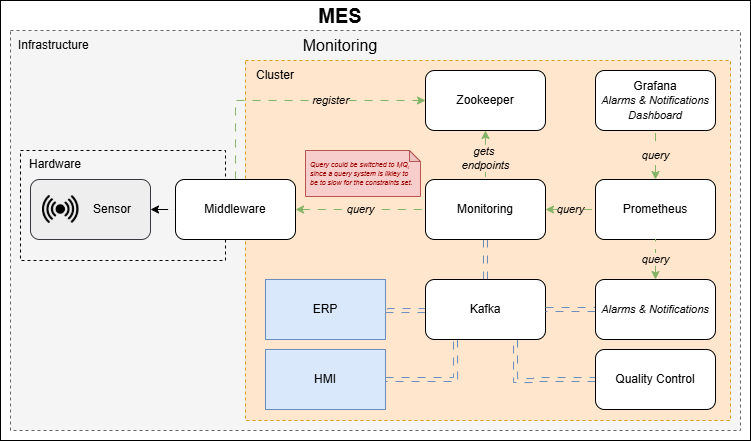
\includegraphics[width=1\linewidth]{report/GroupTemplate/images/MES_monitoring.png}
\end{figure}

\begin{figure}[H]
    \centering
    \caption{A structural diagram showing the structure and communication flow in the \underline{execution} part of the MES subsystem}
    \label{fig:systems_and_subsystems-mes_execution_systemdiagram}
    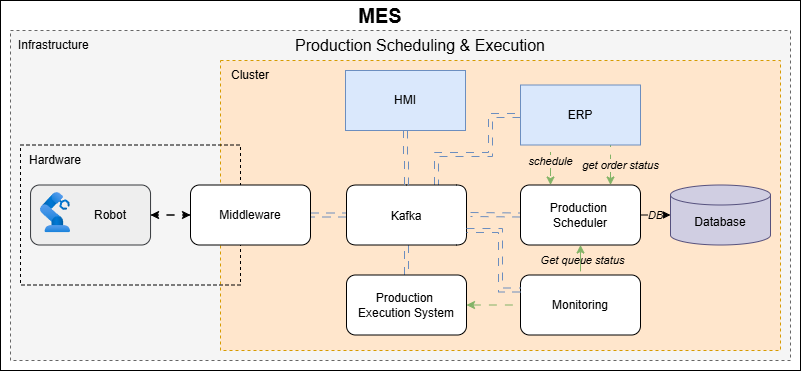
\includegraphics[width=1\linewidth]{report/GroupTemplate/images/mes-execution.png}
\end{figure}

Figure \ref{fig:systems_and_subsystems-mes_execution_systemdiagram} and \ref{fig:systems_and_subsystems-mes_monitoring_systemdiagram} shows together the MES system, in regards to monitoring and production scheduling \& execution.
For the diagrams, blue boxes shows other systems, and white boxes shows subsystems to MES and incorporated existing software system, such as Kafka, Prometheus and Grafana.
The diagram also focuses on the type of transport layer, with blue dotted lines representing queue connection through Kafka, and green representing REST connection with the arrow showing which way the connection were made.
The combined, allows the communication of what elements the MES system is made of, including how existing software can be utilized in the system. Showing how the transport layer is laid out, allows for inspection of integration options, performance and scalability in the system.
The diagrams also show the integration to physical elements, such as sensors and robots, and how communication with them will be handled.


The diagrams for ERP and HMI can be seen in Appendix on Figure \ref{fig:systems_and_subsystems-erp_systemdiagram} and \ref{fig:systems_and_subsystems-hmi_systemdiagram} respectively. A full legend for the diagrams can be seen on Figure \ref{fig:appendix-systems_and_subsystems_legend}. 

\subsection{SysML}
% I lecture4-23-09-2024 & lecture5 - sep 30 kan der læses mere.
% Beskriv hvad det er, og hvordan det bruges i projektet og hvorfor
As stated by Eun-Young Kang:
\begin{quote}
SysML is a graphical modeling language in response to the UML for systems engineering developed by the OMG (Object Management Group). Supports the specification, analysis, design, verification, and validation of systems that include software, hardware, data, and facilities. Intends to specify and architect systems and their components that can then be designed using other domain-specific languages (e.g. UML, AADL, EAST-ADL, etc.) for software design and 3rd party formal  specifications/languages (i.e., timed-automata, promela, modelica, simulink, stateflow, etc.) for formal verification \& validation (V\&V). \cite{EYKlecture4}
\end{quote}

\textbf{Represents:}
\begin{itemize}
    \item "Structural composition, interconnection, and classification;" \cite{EYKlecture4}
    \item "Flow-based, message-based, and state-based behavior;" \cite{EYKlecture4}
    \item "Constraints on the physical and performance properties;" \cite{EYKlecture4}
    \item "Allocations between behavior, structure, and constraints;" \cite{EYKlecture4}
    \item "Requirements and their relationship to other requirements, design elements, and V\&V cases." \cite{EYKlecture4}
\end{itemize}



\subsection{AADL} % MICHAEL
% I lecture4-23-09-2024 er der mere omkring dette
% Beskriv hvad det er, og hvordan det bruges i projektet og hvorfor
AADL (Architecture Analysis and Design Language) is the process of describing a system, on multiple levels. This can be both hardware and software. AADL is also used across engineering disciplines to make sure all engineers on the project, understands the project and what the purpose of the project is.

During the project AADL has been used to create a systematic description of the system, first a description of the overall system were written, then the system were broken down into three systems MES, ERP and HMI. Then each of these systems were defined into even smaller subsystems, see Figure \ref{fig:systems_and_subsystems-system_diagram}. Each of these systems had their own responsibility which is then documented and described. Future work for this process, would be to split the subsystem into even smaller modules with their responsibilities. This is a process that would continue until all the system responsibilities has been accommodated.

%During the project AADL has been used to create a systematic model of the system, as it has described each of the components in section \ref{sec:systems-and-subsystems}. AADL has provided a great understanding of the different components in the system. We chose to have a description of the main systems MES, ERP and HMI. But also an description of each of their subsystems. 

%We could have gone even deeper and described, the different sections in the subsystems, but choose not to do so.

The production line requires high availability with an expected uptime of 24/7, this can be handled with the help of a well-designed architecture. Therefore, by using AADL it is possible to gain insight into which components need high availability at any given time.

% \begin{figure}[H]
%     \centering
%     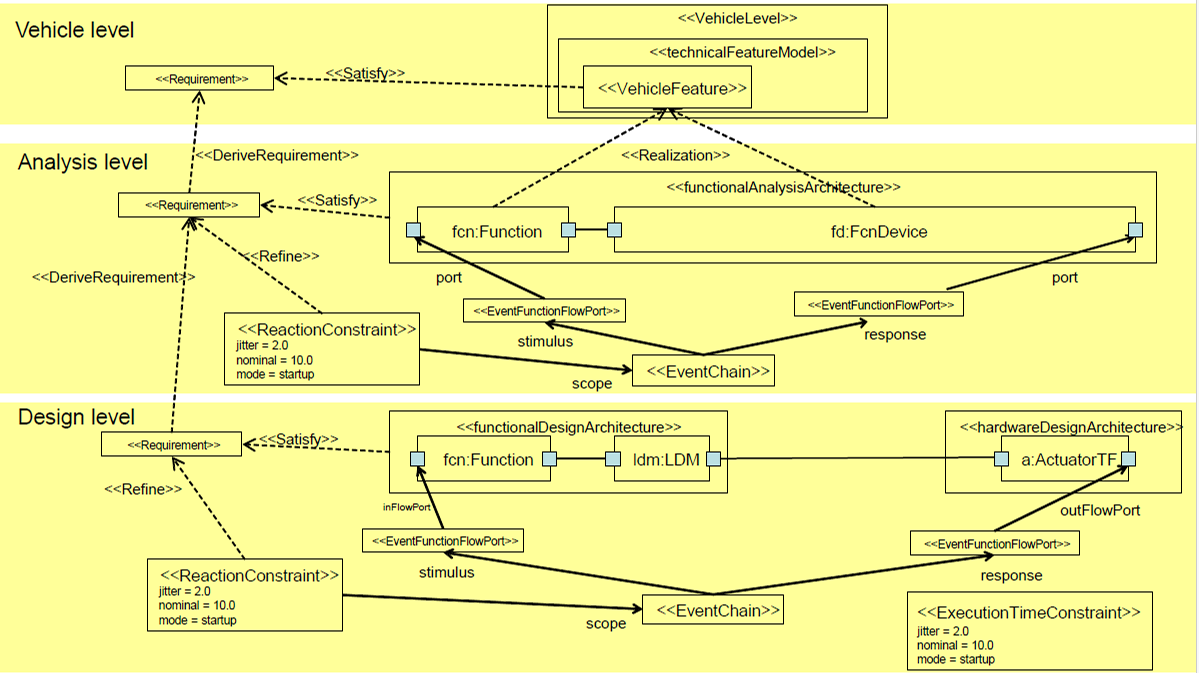
\includegraphics[width=1\linewidth]{report/GroupTemplate/images/formalized constraints.png}
%     \caption{Enter Caption}
%     \label{fig:formalized-contrains-diagram}
% \end{figure}

\subsection{EAST-ADL}
% I lecture4-23-09-2024 er der mere omkring dette
% Beskriv hvad det er, og hvordan det bruges i projektet og hvorfor
This is a guide that help with planning the process of the production line from start to end \cite{eastadl_whitepaper}. This is a process where each stage of the production is meticulously planned and executed.

\begin{figure}[H]
    \centering
    \caption{EAST-ADL Abstraction Levels}
    \label{fig:east-adl-levels}
    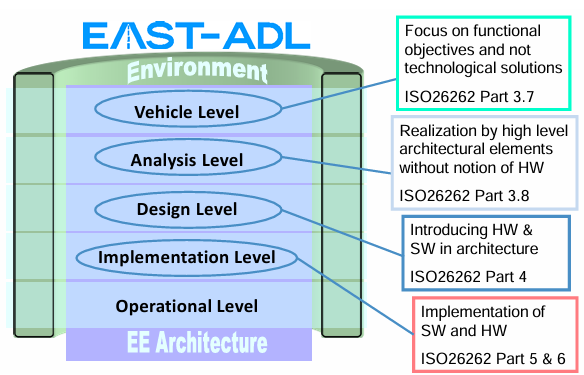
\includegraphics[width=1\linewidth]{report/GroupTemplate/images/EAST-ADL abstraction levels.png}
\end{figure}

Using EAST-ADL, makes it possible to create abstraction at multiple levels, which allows for the design and definition of high-level production goals and refine them into detailed system implementations. By creating a functional decomposition with modular design, it is possible to reuse components across product lines, while integrated traceability ensures that design changes or errors can be easily tracked and resolved.

By using EAST-ADL we ensure that traceability and any errors or inefficiencies in our production line are identified and resolved as quickly as possible, which is important in safety-conscious industries like ours. EAST-ADL’s focus on safety and reliability fits the requirement for the production line to operate safely in a 24/7 environment.

This process also enables the production line to be adapted to different types of ammunition or changes in the market. Furthermore, timing and real-time constraints ensure the synchronization and precision required for manufacturing processes, increasing overall efficiency.

\subsubsection{Vehicle Level}
%high level
%type
%quality standards
%how to oprate safe and effeiciently
This is the top level of the production line with high-level planning. At this level, the goals of the factory are defined, such as what types of ammunition will be produced, what quality standards will be met, and how the factory will operate safely and efficiently. This process is about understanding the big picture and ensuring the production line can produce different types of ammunition while maintaining accuracy and adhering to safety regulations.

\subsubsection{Analysis Level}
%Functions of the production
%what it need to do
%need of sensors to measure and so on
The analysis level is where the functions of the production line are identified and organized. This is about what the production line must do without considering specific machines or technology. The production line will use sensors to measure dimensions, machines to assemble components, and systems to perform quality control. Then each function is analyzed in detail, giving a blueprint of the tasks the production line must perform.

\subsubsection{Design Level}
% Specific tools are chosen
% conveyor belt to transport.
% specific senesors to measure.
% mapping the posistion
The design level is the details of how these functions will be realized. Here, machines and tools are selected and their roles are defined. The conveyor belt for transporting cartridge cases, a robotic arm that applies the projectile, and sensors that provide quality checks are described.
The production line layout is decided, ensuring that all machines and systems are correctly positioned and can communicate effectively with each other.

\subsubsection{Implementation Level}
% Installing the software
% the system is connected and communcate
The implementation level is the level where the production line is brought to life. The machines are installed, the software that controls them is developed and integrated, and the entire system is connected to ensure smooth operation. This could be the production scheduler to control the timing of each step in the production process, ensuring that materials move smoothly from one station to the next, and that errors are detected and corrected in real time.





\subsection{Transport Layer} % Michael. Færdig Skrevet
% Omhandlende de forskellige MQ's, skriv gerne kort pros/conf af de mest gængse.
% På slide lecture_6_middleware er der et fint slide 25 
% læg det billede ind i rapporten, trods det vil se dumt ud, kan det zoomes helt sindsygt.

% SKRIV HER EN FORKLARING AF HVAD TRANSPORT LAYER ER.
% The transport layer is the part that ensures stable and reliable transfer of data between applications. It is an intermediary between the application layer and the network layer.

As the application is built into multiple smaller systems, integrating each system is crucial. A transport layer is introduced to facilitate the transfer of data between each part of the system. 

As the system is very data-oriented, in the form of pulling data from sensors and pushing commands to machines, as well as representing the current actions and states in an HMI, an efficient transport layer is needed. This is especially highlighted by the requirements, which state precision, performance and scalability, as well as availability, is required.

With these aspects, two different approaches to the transport layer are used: Pull-based and push-based.
Pull-based is used when an application needs to retrieve data from another application, and it is in charge of ensuring that it gets the data.
In this system, REST is used as the format for pull-based requests. Soap, GraphQL, gRPC and similar are also viable options and may be introduced by third-party systems. However, providing a uniform API format across the system allows for easier integrations. The use of REST is also most common in the industry, but gRPC may be used where performance and data format are crucial. Therefore REST is the standard in the application, but if critical time-sensitive components are identified in the development phase, they may use gRPC, but the standardized format is REST for its simplicity and ease of use for external- and web-facing services.

Pull-based is not suitable for the whole of the system. As seen in section \ref{sec:architecture-structure-model}, push-based transport is needed.
Push-based communication is based on the notion, that an application wants to push data to other parts of the application that need the data, whereas pull-based based is where applications reach out themself for the data or to trigger actions.
Push-based can be incorporated in three different ways; queues, webhooks and websockets.
However, due to the scale of components that need to interact, queue-based communication is suitable. Queue-based communication allows for a broker to be used. By using a broker, applications that push data do not need to know about whom needs the data, and applications can listen on any queue they want, through the broker. 
Queues also allow for the queuing of messages, while previous data is processed.

Queues therefore provide a scalable system for communicating large volumes of data, using push-based methodologies.

In the system, Kafka has been used as the queue service and broker. Alternatives such as RabbitMQ exist, but Kafka is suitable in this situation, as it is built for high availability, scalability and performance in scaled-up environments.


% HVORFOR BRUGER MAN TRANSPORT LAYEr

% The system is designed with the use of Kafka to handle the transport of data between producers and consumers, it works by producers creating data and consumers using data, this works as a publish and subscribe principle, where producers live with a specific topic, this topic is then used by consumers to receive the relevant data.

% Kafka allows us to decouple the systems from each other which in turn allows for scaling. There has been a focus on principles such as low coupling high cohesion, throughout the process.

% Hvilken type transport layer
% - Push based (queue, websocket)
% - Pull based (Rest, Soap, GraphQL, gRPC, etc.)

% Hvorfor har vi valgt de enkelte teknologier, og hvorfor har vi de to forskellige typer i systemet


% During the project, different transport layers, have been investigated, to ensure that the correct platforms is selected for the project.

% During the project, we have only looked at the different message busses, such as Apache Kafka and RabbitMQ., we haven't looked at the Relational/NoSQL databases for storing other information. 

% Apache Kafka was chosen for the project, as Apache Kafka is ideal for dealing with large amounts of data, where RabbitMQ is suited for moderate amounts of data. And as described in section \textbf{XXX} we expect the system to send large amounts of data. Apache Kafka, is also designed to keep message stored locally. This adds a capability for running old message over and over again, this is good for analysis, troubleshooting, and replay in real-time.  RabbitMQ on the other hand deletes them when the message has been consumed. Apache Kafka keeps the message in sequential order, where RabbitMQ doesn't. This means, that message is always forwards messages Apache Kafka in order, where RabbitMQ doesn't necessarily do it.  
% The downside by using Apache Kafka vs. RabbitMQ is that Apache Kafka is more complex setting up, and requires a lot more management. Where RabbitMQ is more simple to setup, and manage.

% The reason for choosing Apache Kafka in the project, is that the system needs to be running 24/7 and therefore Apache Kafka is more suitable for distributed systems, but it also keeps track of message in a sequential order, which is also important for the factory. Lastly its a nice feature, that it stores all message, such that these can be run again, in case of any trouble shooting on the system.

% Hvorfor er Kafka valgt - Og andre transport muligheder (REST)

\subsection{Containerization} % Skal vi have denne med?
% Hvordan har vi brugt containiraztion (I forhold til deployability)

% Nedenfor er et *meget* groft bud, på hvad afsnittet kunne indeholde. Skal fintunes.
Containerization is a technology that involves packaging an application and its dependencies into an isolated and self-contained container.

Containerization is an important part of the project, as it allows for enhanced deployability. Through the use of Docker as a containerization engine, it is possible to develop and ship software solutions, that run on a larger number of machines, without having to fine-tune each machine to run the software. Orchestration tools like Kubernetes then allow for large-scale deployments, that can live up to stringent availability requirements. 

With the use of Docker and an orchestration tool like Kubernetes, the software is intended to be deployed on multiple machines simultaneously and ensure the software is available 24/7.


\subsection{Programming Language} % SkaL vi have denne med?
Choosing the most suitable language for each subsystem ensures that the system is efficient, easy to maintain and responsive in real-time operations.
% Hvorfor har vi valgt programmerings sprogene i opgaven (argumenter)
% Ikke prioriteret 
% forklar om hvorfor der er forskellige sprog typer
% Types of Programming Languages
    % Machine Language
    % Assembly Language
    % Procedural Programming Language
    % Functional Programming Languages
    % Object-oriented Programming Languages
    % Scripting Languages
    % Logic Programming Language
% De forskellige sprog har deres område

\subsubsection{Real-time sensor data processing and machine control}
\textbf{C++} is highly efficient and works well for applications that require fast response times and precision. It is particularly suitable for handling sensor data and controlling machines on the production line, where low latency is essential for detecting defects and making adjustments in real time.

\subsubsection{Middleware and System Integration (ERP, MES)}
\textbf{Java} is a reliable choice for enterprise applications due to its performance, cross-platform compatibility and scalability. It supports the high throughput requirements of ERP and MES systems, making it ideal for integrating and managing production schedules and inventory in real time.

\subsubsection{Quality control and defect detection}
\textbf{Python} is widely used in machine learning and data analysis, making it ideal for tasks such as defect detection and quality control. Libraries such as OpenCV and TensorFlow simplify the development of AI algorithms for high-accuracy inspections.

\subsubsection{Reporting and real-time dashboards (HMI)}
\textbf{JavaScript (Node.js and React)}, with frameworks like React for the frontend and Node.js for the backend, is perfect for building interactive dashboards and real-time monitoring tools. This setup allows operators to easily view production data, alerts and reports as they happen, ensuring an efficient user experience on the Human-Machine Interface (HMI).

%In the system, there is a focus on using a relevant programming language. However, the major industrial leaders in languages are C\# and Java, which would serve as the main backbone. However, the individual integrations into the different machines may be written in a more specialized language. For example, C\# may be used for windows based integrations, whereas on Linux or other types of machines, Rust, Go or Python may be used if frameworks for this exist.
%However, the design enables the use of different languages, based on the developers and the specific task to undertake. It is however recommended for the backbone, that a well-trusted and structured language is used.

\subsection{Databases}
% Skriv omkring Relationel SQL no NoSQL
% Hvorfor har vi valgt en database model over en anden (Time-series - Prometheus, Mysql, Mongodb, etc.)

The system uses three different kinds of databases; Time-series, relational SQL and document-based NoSQL.

A time-series database is chosen for data that changes in one axis over time, such as sensors. Both SQL and NoSQL is not suitable for time-series, as when data frequency and number of total datapoints stored, reach a certain point, the query time would be too long. Time-series databases, such as InfluxDB and Prometheus, are specifically built for the storage of data streams from sensors and similar.

Relational SQL is used for core elements, such as scheduling, ordering and similar activities where there is a focus on transactional data. For this, databases such as PostgreSQL and MariaDB are often used.

Document-based NoSQL is used, to store larger documents, such as images from image sensors. Document-based NoSQL can also be used to store logs from the system itself. For sensor data, that does not fit in time-series, a database like MongoDB would fit, whereas for logs a database like Elasticsearch is more optimal. However Elasticsearch has a larger focus on search, and image sensor data would be possible to store in Elasticsearch as well, eliminating the requirement for a database like MongoDB. 


\section{Formal Validation and Verification (V\&V)}
\label{sec:formal-v-v}
The validation and verification of an architecture is important to ensure proper evaluation of the architecture. In this chapter we will discuss when to test an architecture along with some tools to formally state and test the logic of a system.

% Formalize the system requirements, including functional properties associate with quality attributes.
% Perform formal verification and simulation to determine if the system meets the specified requirements. Provide the V&V results, along with any counter-examples

% Der er et overview i lecture_1_introduction slide 23

% Fra lecture 10:
% • A list Of requirements verified and its V&V results
% • Are the given properties satisfied? or not-satisfied? If not, describe the reason Of violation based on counter-examples analysis and provide how the current design can be improved/refined based on the V&V results



\subsection{When to Test Architecture} 
% Skriv lidt omkring hvornår man bør teste sin arkitektur, early, late, very late? Står der i lecture_7_evaluating_software_architecture
Evaluation of an architecture is vital to mitigate risks and better ensure project success.

There are some significant points throughout the software development cycle where an evaluation of the architecture can prove crucial. \textit{Early} in the process, when the requirements are not yet fully locked in, a discovery review can be conducted with stakeholders with decision power. This review can be an important help to ensure the architecture being developed are addressing the required quality attributes to satisfy customer needs. \textit{Later} in the development process, when developers begin to make decisions that depend on and are influenced by the system architecture, an evaluation can be held to determine what decisions should be made. This is done when the costs of reverting those decisions outweighs the costs of conducting the evaluation. 
Frameworks for evaluating software in these stages include Architecture Tradeoff Analysis Method (ATAM) for early evaluation to identify business goals and elicit QA requirements and sets of risks, sensitivity- and tradeoff points. Additionally Lightweight Architecture Evaluation (LAE) can more regularly be conducted low-cost and less formally as internal peer reviews, using elements of the ATAM to evaluate changes since the last review.
\textit{Very late}, when the system has largely been implemented, the architecture can be tested and measured to determine whether the architecture fulfills the desired quality attributes. \cite{WormKangLec72024}




\subsection{UPPAAL} 
UPPAAL is a model checker for modeling, validation, and verification of real-time systems. It works using a collection of what is called "networked timed automata" which can be thought of as state-machine diagrams that can communicate with each other. To do model-checking in UPPAAL one needs two things, a model and a requirement specification.
\subsubsection{Model}
The model is a collection of timed and networked automata. As stated above, an automaton (plural: Automata) is based on the idea of a state-machine diagram. It uses a graph-style layout with nodes and edges. These automata describe the behavior of the system.
\subsubsection{Requirement specification}
The requirement specification has two parts which are described by CTL notation (described in section \ref{subsec:CTL})
\begin{itemize}
    \item \textbf{Invariant} (aka. safety property): the requirement that something (bad) never happens. This is often a deadlock where there are no edges to take from a given node so the model is stuck in the current state. But could also be mutual exclusion or and error state.
    \item \textbf{Liveness}: the requirement that something (good) will eventually happen, e.g. a specific state is achieved.
\end{itemize}
% Architecture formal behavior model and RQ specification: Network TA(UPPAAL TA models) and RQ specifications (UPPAAL CTL-quireies) w.r.t. the RQ table

% Det står meget mere om lecture 8 og 9
% Der skal laves UPPAAL CTL queries.


\subsection{Computation Tree Logic}
\label{subsec:CTL}
Computation Tree Logic (CTL) can be seen as a language for asking questions regarding a system. You can use CTL to ask "What will happen in the future", or "Is something always true". The system can be both hardware, software or a combination. CTL is used to describe what a component does and doesn't.

\begin{equation*}
    AX (red \rightarrow green)
\end{equation*}

\subsubsection{CTL Example}
Imagine a traffic light system managing the north-south direction. It can have two possible states:
\begin{itemize}
    \item \textbf{NS\_red}: The light is red for north-south traffic.
    \item \textbf{NS\_green}: The light is green for north-south traffic.
\end{itemize}
We want to ensure that "The north-south light must remain red until it turns green".
The CTL Formula for this CTl is
\begin{equation*}
    E (NS\_red \cup NS\_green)
\end{equation*}
Explanation:
\begin{itemize}
    \item \textbf{NS\_red} must remain true as long as the light has not turned green. 
    \item The system will eventually reach a state where \textbf{NS\_green} is true, and the requirement stops.
\end{itemize}



\begin{figure}[H]
    \centering
    \caption{An explainer for path qualifiers and linear temporal operators in CTL}
    \label{fig:ctl-pq_and_lto_cheatsheet}
    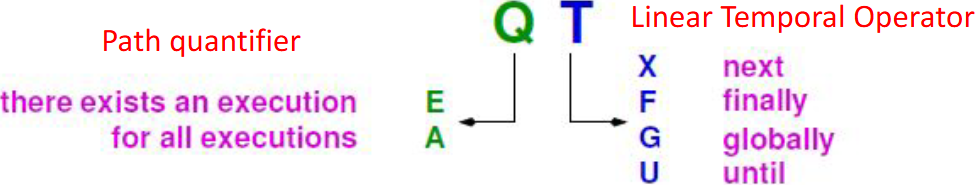
\includegraphics[width=1\linewidth]{report/GroupTemplate/images/ctl-notatio_explainer.png}
\end{figure}

A CTL statement is build up by Path Quantifier and Linear Temporal Operators. We always need to have at least one Path Quantifier and one Linear Temporal Operator. 

%If we are missing the Path Quantifier the statement, doesnt say anything about if we are talking about all paths, or just a single one. And for Liniar Temporal Operators, it's also required to have atleast one, 

\subsubsection{Path qualifier (PQ)}
Path qualifiers are used to describe the scope of the CTL-formula. %If e.g. we are dont include a PQ, there statement will no longer say anything about which path is the one we are working. 
\begin{itemize}
    \item \textbf{E}: There exists at least one path
    \item \textbf{A}: For all possible paths
\end{itemize}

\subsubsection{Liniar Temporal Operators (LTO)}
Liniar temporal operators describe in what scenario the following statement needs to be true
\begin{itemize}
    \item \textbf{X}: Next - true in next state
    \item \textbf{F}: Finally - true in any future state
    \item \textbf{G}: Globally - true in all future states
    \item \textbf{U}: Until - true until a different state is true
\end{itemize}
% Explain what LTO is

\medskip

How CTL works: A system can have multiple paths or scenarios (lets call them roads), imagine.
\begin{itemize}
    \item[] You standing at a road, and there is multiple intersection in front of you.
    \item[] Each road represents a future state of the system.
\end{itemize}
With CTL you can ask some of the following questions.
\begin{itemize}
    \item[] "Can I always go left?"
    \item[] "Can I get to my destination by \textbf{one or another read}?"
    \item[] "What happens, \textbf{no matter which road I take}?"
\end{itemize}

\medskip








\section{Evaluation}
\label{sec:evaluation}
%Forklar kort hvad evaluering er og hvorfor det er vigtigt at evaluere på det som er lavet.
% Describe the evaluation design, measurements of the QASes, pilot test, and an analysis of the results. Describe the design for the evaluation, measurements of the QASes, pilot test, and an analysis of the results. From the analysis, how it answers the research questions must be clear
To evaluate the process we have been through, it is important to analyze whether the requirements and goals that have been defined have been answered throughout the process. It is important to evaluate in the areas that have been defined based on our research questions, which are our focus area.
% Forklar om experiment (resultater) -> Flyt experiment her
The following experiment is a experiment answering the research questions in \ref{sec:research-question}


\subsection{System Experimentation}
% Forklar om experiment (hvordan)
% Introducere experiment
Due to a production line that demands quality attributes such as performance, integrability, modifiability and availability, it is necessary to validate whether the sensor data generated can reach the modules that need the data, efficiently and reliably to act. Therefore, the experiment is built around Kafka's ability to transport messages across the system quickly and reliably and with different amounts of sensors due to the requirement to be able to scale.

In order to conduct a test, the \textbf{Goal-Question-Metric (GQM) framework} was used.

%GQM
\textbf{Goal}: production efficiently precess data in real-time.

\textbf{Questions}:
\begin{itemize}
    \item How quickly can anomalies be detected and communicated to Production Environment systems (PES)?
    \item How scalable is the solution for multiple production lines?
\end{itemize}
\textbf{Metrics}: Latency (milliseconds), throughput (events/sec), and anomaly detection accuracy.

%Methodology
The method for carrying out the experiment is based on creating a pipeline where real-time sensor data is streamed and collected by modules that use this data.

%Hypothesis
In order to evaluate this, the following \textbf{hypotheses} are made.

\textbf{Low Latency Hypothesis}
\begin{itemize}
    \item \( H_0 \): Kafka cannot maintain low latency (\(< 5 \, \text{ms}\)) for real-time data processing under industrial-scale workloads.
    \item \( H_1 \): Kafka can maintain low latency (\(< 5 \, \text{ms}\)) for real-time data processing under industrial-scale workloads.
\end{itemize}
\textbf{Scalability Hypothesis}:
\begin{itemize}
    \item \( H_0 \): Kafka’s performance deteriorates significantly as the volume of data streams increases (e.g., latency exceeding \(10 \, \text{ms}\)).
    \item \( H_1 \): Kafka’s performance scales efficiently with increasing data volumes, maintaining consistent latency and throughput.
\end{itemize}
%Data collection & Validation
The produced data was saved in CSV files to be analyzed using various graphs. The data was collected by running the experiment five times with different workload levels where the amount of events/per sec was increased.


%Limitations
However, there are also limitations that affect the validity of the experiment, as the experiment was conducted in a simulated environment, which therefore cannot be compared to how it would function in a real-time environment.

%Conclusion & future work
The result showed that it was possible to prove the given hypotheses, since it was possible to have a latency ($<5\,\text{ms}$) and high throughput ($>1{,}000\,\text{events/sec}$). Therefore, it is possible for Kafka to comply with scalability, reliability and safety as it can send alarm messages across the system within ($<5\,\text{ms}$).

Future work will explore scalability across multi-line production setups, improve latency under higher data loads, and evaluate performance in real-world industrial environments.




\section{Discussion}
\label{sec:discussion}
% punkterne fra sidste slide i Asaa_exercise_10_slides skal alle diskuteres her.

This section will highlight some key aspects of Formal V\&V, why it is used and when, as well as the use of experimental evaluation. At last, it will also highlight why formal design is necessary.

\subsection{The Importance of Formal V\&V Before System Implementation}
% The Importance of Formal V&V Before System Implementation: Explain why formal Verification and Validation (V&V) is crucial before implementing a system

Developing a larger system is often a lengthy and expensive process. By doing V\&V it is possible to reduce the risk, that a large project introduces, in regard to its design and structure. 
By using methods such as UPPAAL, it is possible to validate that processes are possible and optimal. By mapping and modelling system architecture and components in its different forms, blind spots are uncovered and can be corrected.


\subsection{Comparing Formal V\&V and Experimental Evaluation}
% Comparing Formal V&V and Experimental Evaluation: Discuss the relationships and differences between formal V&V and the experimental evaluation of the system

Formal V\&V is different from experimental evaluation, as formal V\&V is done theoretically and in simulations. Therefore, no real code that can be used is produced. The system in evaluation is put in a vacuum per se. The structure of the system is evaluated, and the behaviour is modelled.
In experimental evaluation, the focus is on real-world experimentation, where code is being written. However, the code may be limited and restricted. It allows us to test real software issues and see if frameworks and areas that are less understood for the project, are to be explored.
Experimental evaluation therefore focuses on a closer example to the real software and tests the hypothesis created for the system to be built or being built. However, Experimental evaluation can be time-consuming, and not be able to mimic all aspects of the final product, as it will always be a subpart of the final product.
Experimental evaluation may also use methods such as Software-in-the-loop (SIL) or Hardware-in-the-loop (HIL), which allows the built software to be tested against simulated environments (either through software simulation, SIL, or through hardware simulation, HIL). This allows for code to be tested against known scenarios, and test to see if the software can handle different scenarios. However, these methods are used in the development phase, to faster test software against complex scenarios, but could be used in the evaluation of architecture on small-scale prototype code.
% SIL: https://www.aptiv.com/en/insights/article/what-is-software-in-the-loop-testing
% HIL: https://www.aptiv.com/en/insights/article/what-is-hardware-in-the-loop-testing

The two methods therefore represent two sides of validation, as one focuses on theory and simulations, and the other focuses on a closer to reality, but more time-consuming and limited testing.

\subsection{Necessities of Formal Design and Analysis and Its Benefits}
% Necessities of Formal Design and Analysis: Highlight the need for formal design and analysis, including V&V, before experimental evaluation (e.g., Software-in-the-Loop (SIL), Hardware-in-the-Loop (HIL))

Before moving to experimental evaluations, either using prototype code and testing the hypothesis of the architecture or by using SIL and HIL methods, formal design an analysis, as well as V\&V is a crucial step. 
The design, analysis and V\&V provide a base, in which the architecture and software can be built. Ensuring the software is well designed, and done so on an analysis, allows for the architecture to be well structured and provide a good development life cycle. Without a proper design, built on formal designs and analysis, the software may be built incorrectly, which could end up costing a large sum and time to correct at a later stage. 
Therefore, doing design early, and on an objective basis, allows for catching errors early and correcting them while it is possible without impacting the total cost and timeline of the project.


% \subsection{Benefits of V\&V}
% Benefits of V&V: Discuss the benefits of using V&V in system development

% The use of V\&V througout the system development, is important, as it allows the developers to take an objective view of the system. It gives a way to formally validate the system, and ensure it lives up to the requirements. Without formal validation and verification, much of the reasoning behind a given architecture in subjective and based on personal experience. 



\section{Conclusion}
\label{sec:conclusion}
% - Summary of the work and result.
% Discuss how the work can be extended with respect to the approach and/or evaluation

The project involved creating a system architecture for an ammunition production line, emphasizing the use of appropriate tools to execute the project systematically and in a structured manner. Based on the research questions posed, a literature review was conducted to examine previous studies in the field. The focus was on addressing the research questions defined in Section \ref{sec:research-question} by analyzing insights from related studies. Throughout the process, the questions were answered using a systematic architectural model and experiments, which demonstrated the system's ability to scale while maintaining low latency and high availability in the simulated environment. However, further work is required to validate the architecture in a real-time environment.



\newpage


\bibliographystyle{IEEEtran}
\bibliography{report/GroupTemplate/references}

% \newpage
%  .

\newpage

\section{Appendix}
\label{sec:appendix}
% Max of 2 pages

\begin{figure}[H]
    \centering
    \caption{A structural diagram showing the structure and communication flow in the ERP subsystem}
    \label{fig:systems_and_subsystems-erp_systemdiagram}
    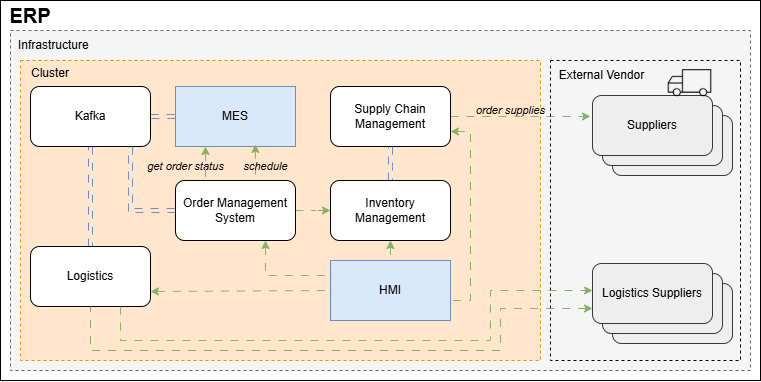
\includegraphics[width=0.9\linewidth]{report/GroupTemplate/images/erp_subsystem.png}
\end{figure}

\begin{figure}[H]
    \centering
    \caption{A structural diagram showing the structure and communication flow in the HMI subsystem}
    \label{fig:systems_and_subsystems-hmi_systemdiagram}
    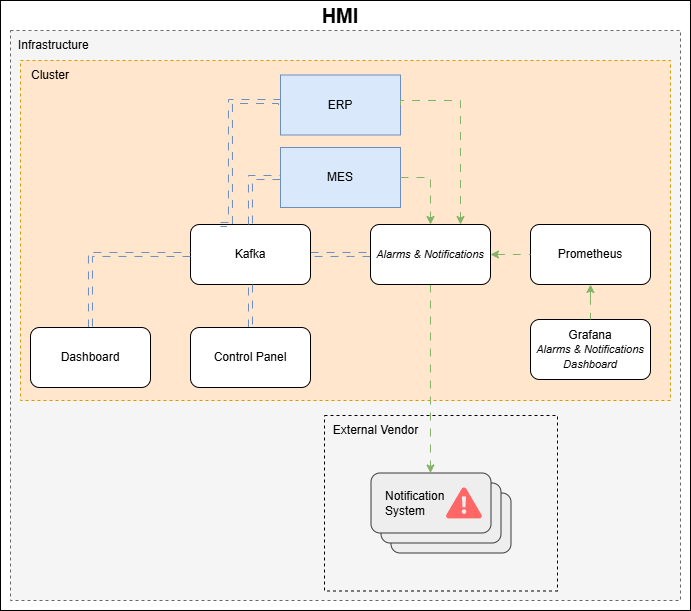
\includegraphics[width=0.9\linewidth]{report/GroupTemplate/images/HMI_subsystem.png}
\end{figure}

\begin{figure}[H]
    \centering
    \caption{The Legend for All Structural Diagrams}
    \label{fig:appendix-systems_and_subsystems_legend}
    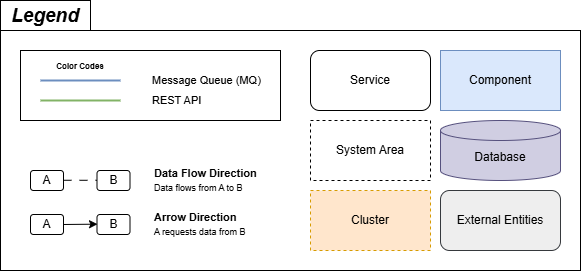
\includegraphics[width=0.9\linewidth]{report/GroupTemplate/images/systems_subsystems-legend.png}
\end{figure}

\begin{figure}[H]
    \centering
    \caption{Use Case UC01}
    \label{fig:appendix-use-case-01}
    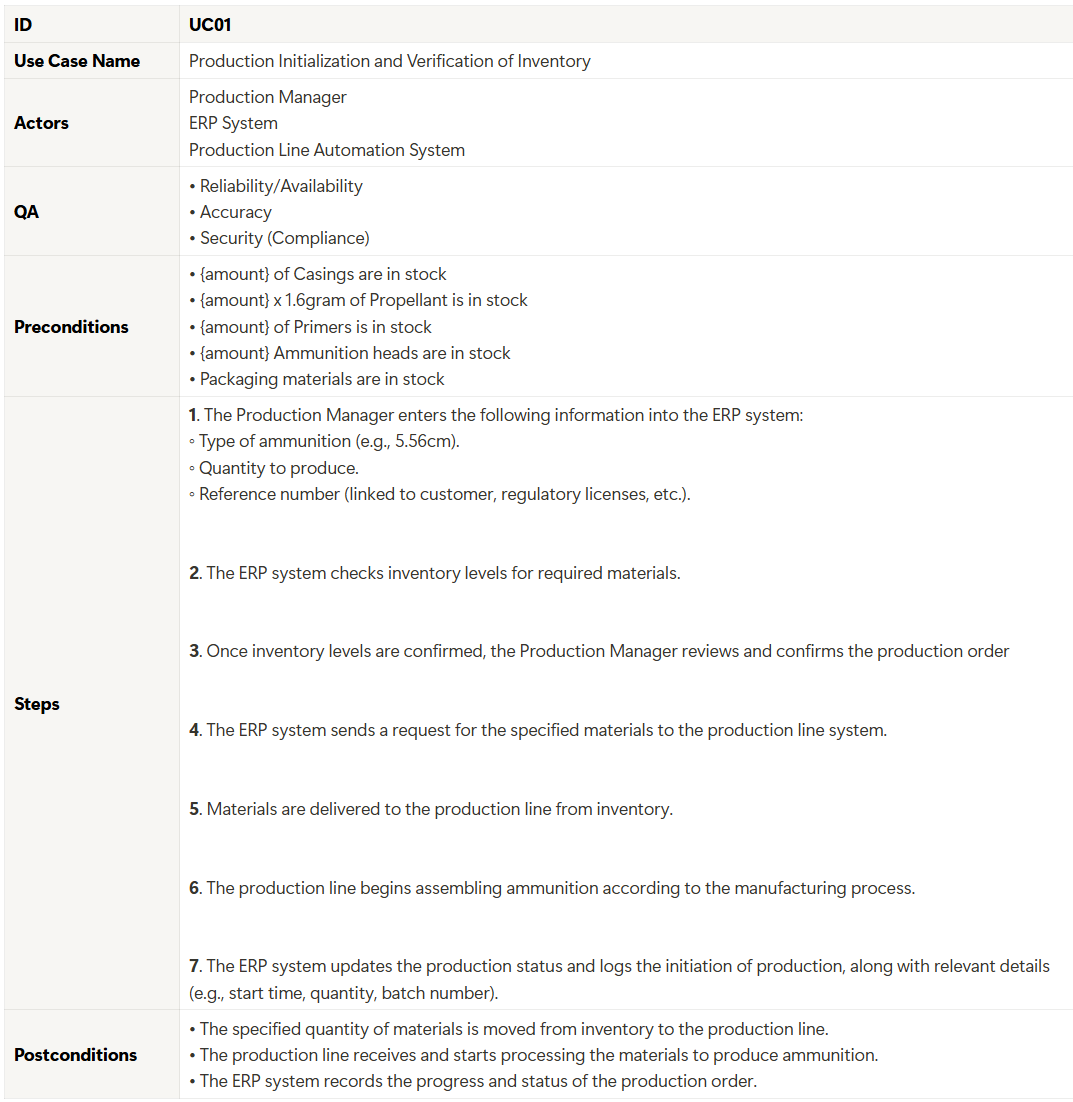
\includegraphics[width=0.9\linewidth]{report/GroupTemplate/images/usecase-01.png}
\end{figure}

\begin{figure}[H]
    \centering
    \caption{Structural Diagram - Overview of Different Diagrams}
    \label{fig:structural-diagram}
    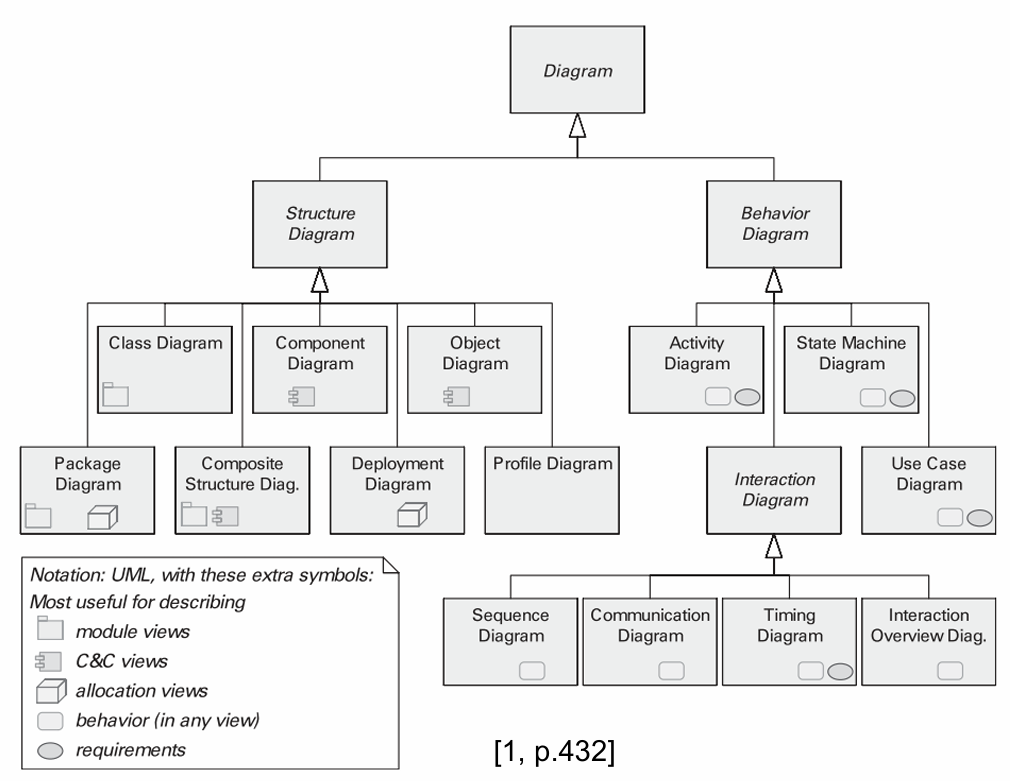
\includegraphics[width=0.9\linewidth]{report/GroupTemplate/images/structual diagram.png}
\end{figure}


%\input{report/GroupTemplate/chapters/0 Abstract}

%\input{report/GroupTemplate/chapters/1 Introduction}

%\input{report/GroupTemplate/chapters/2 Diagrams}

%\input{report/GroupTemplate/chapters/3 Requirements}

%\input{report/GroupTemplate/chapters/4 Quality Attributes}

%\input{report/GroupTemplate/chapters/5 System Overview}



%\input{report/GroupTemplate/chapters/7 FORMAL VERIFICATION AND VALIDATION}

%\input{report/GroupTemplate/chapters/8 Discussion}

%\input{report/GroupTemplate/chapters/9 Conclusion}



%0 Abstract

%1 Introduction

%2 Diagrams 
%    use Case
%    Sequence Diagram


%3 Requirements

%    Requirements Diagram

%4 QA

%5 System overview

%Tag billedet fra slide 5 i præsentationen. Forklaring omkring de forskellige systemet og forklar hvordan de kommunikerer med hinanden.

%    Over all diagram
    
%    HMI Diagram

%    ERP Diagram

%    MES Diagram




%7 FORMAL VERIFICATION AND VALIDATION (V\&V)
%    Testings (Jons kode)

%8 Diskution

%9 Konklusion

